\section{Excecution of an analysis}
\label{analysisexcecution}
The execution of an analysis is assigned to the analysis window.\\
From the main window of Romeo, select the \textit{Start Analysis} button or choose the right one in the toolbar (see \ref{environment}). The analysis window (fig. \ref{analysisimg}), is composed of two panels. The left one contains a drop-down menu, that allow the user to select the Dataset\g{} of interest. The right one contains an area in which Romeo will show the feature extractors\g{} associated with the selected Dataset\g{}. The user can choose which results of the extraction will be saved and/or shown during the analysis, checking the feature extractors\g{} of interest shown in the right panel. In any moment, the user can go back to the main window by selecting the \textit{Back} button.
\begin{figure}[!h]
\begin{center}
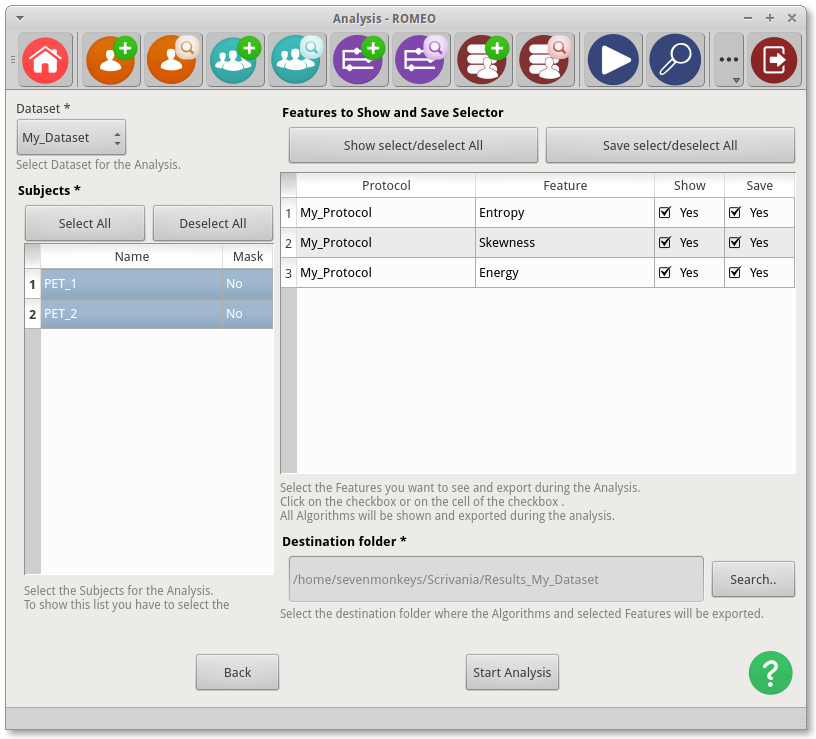
\includegraphics[scale=0.4]{./Images/StartAnalysis}
\caption{\textit{Analysis window}}
\label{analysisimg}
\end{center}
\end{figure}
\\To execute an analysis, follow these instructions:
\begin{itemize}
\item From the analysis window, select the Dataset\g{} of interest from the drop-down menu;
\item Select the Subjects\g{} that you want to analyze from the list in the left panel;
\item Check which results of the feature extractors\g{} will be shown and/or saved in the right panel;
\item Select the \textit{Search..} button to indicate the destination folder of the analysis results;
\item Select the \textit{Start Analysis} button.
\end{itemize}
During the analysis, a pop up window will show the progress of the computation and in addition the results of the feature extractors\g{} if selected before. You can navigate through the results with the \textit{Previous} and \textit{Next} buttons (see fig.\ref{analysisprogress}).
\begin{figure}[!h]
\begin{center}
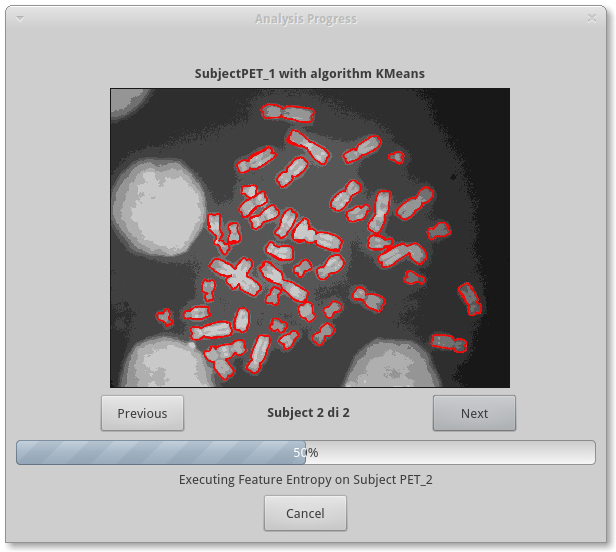
\includegraphics[scale=0.4]{./Images/AnalysisProgress}
\caption{\textit{Progression of an analysis}}
\label{analysisprogress}
\end{center}
\end{figure}
\pagebreak